\begin{figure}[H]
    \begin{subfigure}[t]{0.5\textwidth}
        \centering
        \begin{adjustbox}{max width=0.49\textwidth}
            \centering
            % Scale factor 0.12470588235294117
\definecolor{color15}{RGB}{255,255,255}
\definecolor{color16}{RGB}{255,255,153}
\definecolor{color17}{RGB}{153,255,153}
\definecolor{color18}{RGB}{0,150,60}
\definecolor{color19}{RGB}{0,0,0}
% Bounding Box: 235.0, 170.0
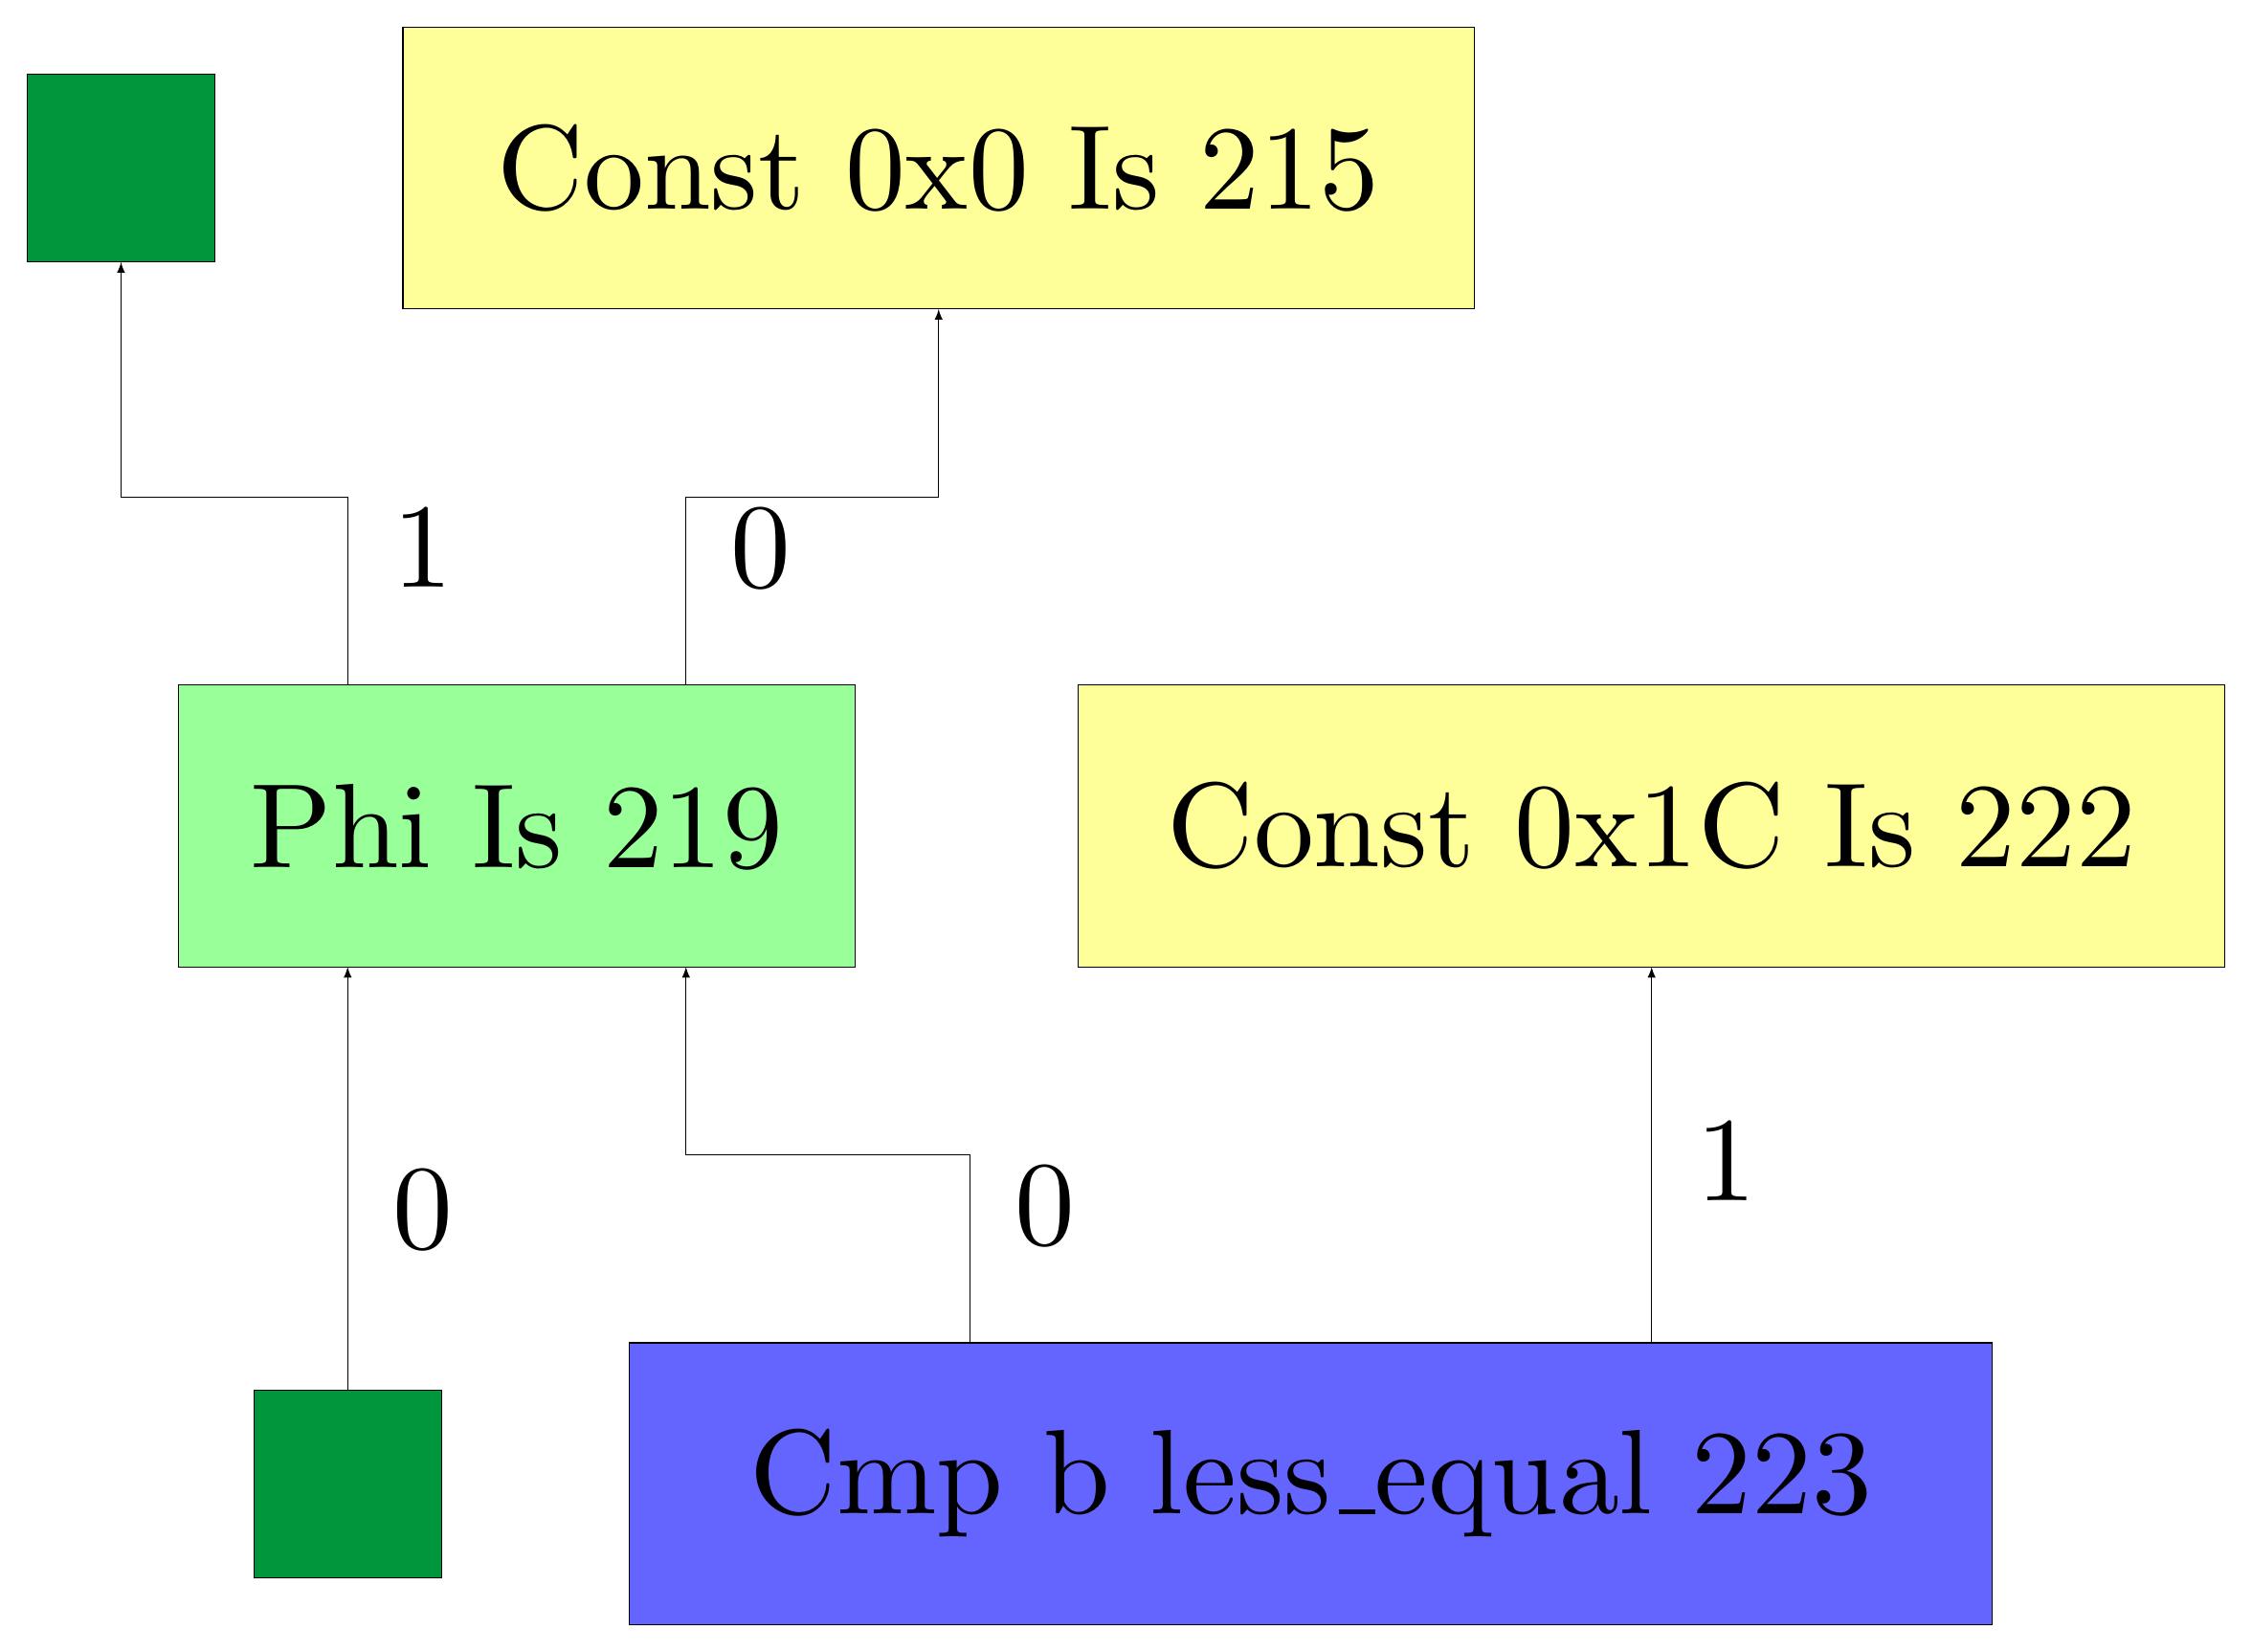
\begin{tikzpicture}
	\node[fill=color15, draw, minimum width=18.08235294117647cm, minimum height=3.741176470588235cm] (n57) at (37.13667820069204cm ,-51.37882352941176cm) {};
	% 1 node layouts
	\node[scale=4.5347593582887695, transform shape] at (37.13667820069204cm ,-51.37882352941176cm) {Cmp b less\_equal 223};
	\node[fill=color16, draw, minimum width=15.214117647058822cm, minimum height=3.741176470588235cm] (n58) at (41.65726643598616cm ,-42.64941176470588cm) {};
	% 1 node layouts
	\node[scale=4.5347593582887695, transform shape] at (41.65726643598616cm ,-42.64941176470588cm) {Const 0x1C Is 222};
	\node[fill=color17, draw, minimum width=8.978823529411764cm, minimum height=3.741176470588235cm] (n59) at (26.59903114186851cm ,-42.64941176470588cm) {};
	% 1 node layouts
	\node[scale=4.5347593582887695, transform shape] at (26.59903114186851cm ,-42.64941176470588cm) {Phi Is 219};
	\node[fill=color16, draw, minimum width=14.216470588235293cm, minimum height=3.741176470588235cm] (n60) at (32.196124567474044cm ,-33.919999999999995cm) {};
	% 1 node layouts
	\node[scale=4.5347593582887695, transform shape] at (32.196124567474044cm ,-33.919999999999995cm) {Const 0x0 Is 215};
	\node[fill=color18, draw, minimum width=2.4941176470588236cm, minimum height=2.4941176470588236cm] (n61) at (24.354325259515573cm ,-51.37882352941176cm) {};
	\node[fill=color18, draw, minimum width=2.4941176470588236cm, minimum height=2.4941176470588236cm] (n62) at (21.346712802768167cm ,-33.919999999999995cm) {};
	\draw[color=color19, -latex] (32.616089965397926cm ,-49.50823529411764cm) -- (32.616089965397926cm ,-47.01411764705882cm) -- (28.843737024221454cm ,-47.01411764705882cm) -- (28.843737024221454cm ,-44.519999999999996cm);
	\node[] at (33.61373702422145cm ,-47.69220588235294cm) {
		\scalebox{4.5347593582887695}{0}
	};
	\draw[color=color19, -latex] (41.65726643598616cm ,-49.50823529411764cm) -- (41.65726643598616cm ,-44.519999999999996cm);
	\node[] at (42.65491349480969cm ,-47.114954044117646cm) {
		\scalebox{4.5347593582887695}{1}
	};
	\draw[color=color19, -latex] (28.843737024221454cm ,-40.77882352941176cm) -- (28.843737024221454cm ,-38.28470588235294cm) -- (32.196124567474044cm ,-38.28470588235294cm) -- (32.196124567474044cm ,-35.790588235294116cm);
	\node[] at (29.841384083044982cm ,-38.96279411764706cm) {
		\scalebox{4.5347593582887695}{0}
	};
	\draw[color=color19, -latex] (24.354325259515573cm ,-40.77882352941176cm) -- (24.354325259515573cm ,-38.28470588235294cm) -- (21.346712802768167cm ,-38.28470588235294cm) -- (21.346712802768167cm ,-35.16705882352941cm);
	\node[] at (25.3519723183391cm ,-38.96279411764706cm) {
		\scalebox{4.5347593582887695}{1}
	};
	\draw[color=color19, -latex] (24.354325259515573cm ,-50.13176470588235cm) -- (24.354325259515573cm ,-44.519999999999996cm);
	\node[] at (25.3519723183391cm ,-47.738483455882346cm) {
		\scalebox{4.5347593582887695}{0}
	};
\end{tikzpicture}

        \end{adjustbox}
        \caption{The original condition with bound $N$}
    \end{subfigure}
    \begin{subfigure}[t]{0.5\textwidth}
        \centering
        \begin{adjustbox}{max width=0.49\textwidth}
            \centering
            % Scale factor 0.010830324909747292
\definecolor{color8}{RGB}{192,192,192}
\definecolor{color9}{RGB}{255,255,255}
\definecolor{color10}{RGB}{153,255,153}
\definecolor{color11}{RGB}{255,255,153}
\definecolor{color12}{RGB}{153,153,255}
\definecolor{color13}{RGB}{0,150,60}
\definecolor{color14}{RGB}{0,0,0}
\definecolor{color15}{RGB}{100,100,255}
% Bounding Box: 1385.0, 2288.0
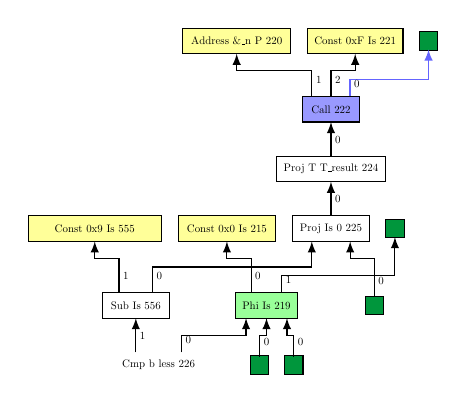
\begin{tikzpicture}
	% 1 node layouts
	\node[scale=0.39382999671808333, transform shape] at (18.93490027571706cm ,15.87725631768953cm) {Cmp b less 226};
	\node[fill=color10, draw, minimum width=0.779783393501805cm, minimum height=0.3249097472924188cm] (n20) at (20.304936376800093cm ,16.63537906137184cm) {};
	% 1 node layouts
	\node[scale=0.39382999671808333, transform shape] at (20.304936376800093cm ,16.63537906137184cm) {Phi Is 219};
	\node[fill=color11, draw, minimum width=1.2346570397111913cm, minimum height=0.3249097472924188cm] (n21) at (19.802367645892012cm ,17.610108303249095cm) {};
	% 1 node layouts
	\node[scale=0.39382999671808333, transform shape] at (19.802367645892012cm ,17.610108303249095cm) {Const 0x0 Is 215};
	\node[fill=color9, draw, minimum width=0.855595667870036cm, minimum height=0.3249097472924188cm] (n22) at (18.64518908438132cm ,16.63537906137184cm) {};
	% 1 node layouts
	\node[scale=0.39382999671808333, transform shape] at (18.64518908438132cm ,16.63537906137184cm) {Sub Is 556};
	\node[fill=color11, draw, minimum width=1.6895306859205776cm, minimum height=0.3249097472924188cm] (n23) at (18.12366728488118cm ,17.610108303249095cm) {};
	% 1 node layouts
	\node[scale=0.39382999671808333, transform shape] at (18.12366728488118cm ,17.610108303249095cm) {Const 0x9 Is 555};
	\node[fill=color9, draw, minimum width=0.9747292418772563cm, minimum height=0.3249097472924188cm] (n24) at (21.12366728488118cm ,17.610108303249095cm) {};
	% 1 node layouts
	\node[scale=0.39382999671808333, transform shape] at (21.12366728488118cm ,17.610108303249095cm) {Proj Is 0 225};
	\node[fill=color9, draw, minimum width=1.3754512635379061cm, minimum height=0.3249097472924188cm] (n25) at (21.12366728488118cm ,18.368231046931406cm) {};
	% 1 node layouts
	\node[scale=0.39382999671808333, transform shape] at (21.12366728488118cm ,18.368231046931406cm) {Proj T T\_result 224};
	\node[fill=color12, draw, minimum width=0.7256317689530686cm, minimum height=0.3249097472924188cm] (n26) at (21.12366728488118cm ,19.126353790613717cm) {};
	% 1 node layouts
	\node[scale=0.39382999671808333, transform shape] at (21.12366728488118cm ,19.126353790613717cm) {Call  222};
	\node[fill=color11, draw, minimum width=1.3646209386281587cm, minimum height=0.3249097472924188cm] (n27) at (19.925875004958936cm ,19.9927797833935cm) {};
	% 1 node layouts
	\node[scale=0.39382999671808333, transform shape] at (19.925875004958936cm ,19.9927797833935cm) {Address \&\_n P 220};
	\node[fill=color11, draw, minimum width=1.2129963898916967cm, minimum height=0.3249097472924188cm] (n28) at (21.43129016741381cm ,19.9927797833935cm) {};
	% 1 node layouts
	\node[scale=0.39382999671808333, transform shape] at (21.43129016741381cm ,19.9927797833935cm) {Const 0xF Is 221};
	\node[fill=color13, draw, minimum width=0.21660649819494585cm, minimum height=0.21660649819494585cm] (n29) at (20.651506773912008cm ,15.87725631768953cm) {};
	\node[fill=color13, draw, minimum width=0.21660649819494585cm, minimum height=0.21660649819494585cm] (n30) at (21.935941653112227cm ,17.610108303249095cm) {};
	\node[fill=color13, draw, minimum width=0.21660649819494585cm, minimum height=0.21660649819494585cm] (n31) at (22.36269810965208cm ,19.9927797833935cm) {};
	\node[fill=color13, draw, minimum width=0.21660649819494585cm, minimum height=0.21660649819494585cm] (n32) at (21.674972477883124cm ,16.63537906137184cm) {};
	\node[fill=color13, draw, minimum width=0.21660649819494585cm, minimum height=0.21660649819494585cm] (n33) at (20.218293777522113cm ,15.87725631768953cm) {};
	\draw[color=color14, -latex] (19.2246114670528cm ,16.03971119133574cm) -- (19.2246114670528cm ,16.256317689530686cm) -- (20.045008578966158cm ,16.256317689530686cm) -- (20.045008578966158cm ,16.47292418772563cm);
	\node[] at (19.31125406633078cm ,16.197427797833935cm) {
		\scalebox{0.39382999671808333}{0}
	};
	\draw[color=color14, -latex] (18.64518908438132cm ,16.03971119133574cm) -- (18.64518908438132cm ,16.47292418772563cm);
	\node[] at (18.731831683659298cm ,16.247560356498195cm) {
		\scalebox{0.39382999671808333}{1}
	};
	\draw[color=color14, -latex] (20.109990528424643cm ,16.79783393501805cm) -- (20.109990528424643cm ,17.231046931407942cm) -- (19.802367645892012cm ,17.231046931407942cm) -- (19.802367645892012cm ,17.447653429602887cm);
	\node[] at (20.19663312770262cm ,17.005683100180505cm) {
		\scalebox{0.39382999671808333}{0}
	};
	\draw[color=color14, -latex] (20.499882225175543cm ,16.79783393501805cm) -- (20.499882225175543cm ,17.014440433212997cm) -- (21.935941653112227cm ,17.014440433212997cm) -- (21.935941653112227cm ,17.501805054151625cm);
	\node[] at (20.586524824453523cm ,16.955550541516246cm) {
		\scalebox{0.39382999671808333}{1}
	};
	\draw[color=color14, -latex] (18.85908800134883cm ,16.79783393501805cm) -- (18.85908800134883cm ,17.122743682310468cm) -- (20.879984974411865cm ,17.122743682310468cm) -- (20.879984974411865cm ,17.447653429602887cm);
	\node[] at (18.945730600626806cm ,17.005683100180505cm) {
		\scalebox{0.39382999671808333}{0}
	};
	\draw[color=color14, -latex] (18.43129016741381cm ,16.79783393501805cm) -- (18.43129016741381cm ,17.231046931407942cm) -- (18.12366728488118cm ,17.231046931407942cm) -- (18.12366728488118cm ,17.447653429602887cm);
	\node[] at (18.51793276669179cm ,17.005683100180505cm) {
		\scalebox{0.39382999671808333}{1}
	};
	\draw[color=color14, -latex] (21.12366728488118cm ,17.772563176895307cm) -- (21.12366728488118cm ,18.205776173285198cm);
	\node[] at (21.21030988415916cm ,17.98041234205776cm) {
		\scalebox{0.39382999671808333}{0}
	};
	\draw[color=color14, -latex] (21.12366728488118cm ,18.530685920577618cm) -- (21.12366728488118cm ,18.96389891696751cm);
	\node[] at (21.21030988415916cm ,18.73853508574007cm) {
		\scalebox{0.39382999671808333}{0}
	};
	\draw[color=color14, -latex] (20.881790028563493cm ,19.28880866425993cm) -- (20.88179002856349cm ,19.613718411552345cm) -- (19.925875004958936cm ,19.613718411552345cm) -- (19.925875004958936cm ,19.83032490974729cm);
	\node[] at (20.96843262784147cm ,19.496657829422382cm) {
		\scalebox{0.39382999671808333}{1}
	};
	\draw[color=color14, -latex] (21.12366728488118cm ,19.28880866425993cm) -- (21.12366728488118cm ,19.613718411552345cm) -- (21.43129016741381cm ,19.613718411552345cm) -- (21.43129016741381cm ,19.83032490974729cm);
	\node[] at (21.21030988415916cm ,19.496657829422382cm) {
		\scalebox{0.39382999671808333}{2}
	};
	\draw[color=color15, -latex] (21.36554454119887cm ,19.28880866425993cm) -- (21.36554454119887cm ,19.505415162454874cm) -- (22.36269810965208cm ,19.505415162454874cm) -- (22.36269810965208cm ,19.884476534296027cm);
	\node[] at (21.45218714047685cm ,19.446525270758123cm) {
		\scalebox{0.39382999671808333}{0}
	};
	\draw[color=color14, -latex] (20.651506773912008cm ,15.985559566787003cm) -- (20.651506773912008cm ,16.256317689530686cm) -- (20.564864174634028cm ,16.256317689530686cm) -- (20.564864174634028cm ,16.47292418772563cm);
	\node[] at (20.738149373189984cm ,16.170351985559567cm) {
		\scalebox{0.39382999671808333}{0}
	};
	\draw[color=color14, -latex] (21.674972477883124cm ,16.743682310469314cm) -- (21.674972477883124cm ,17.231046931407942cm) -- (21.367349595350493cm ,17.231046931407942cm) -- (21.367349595350493cm ,17.447653429602887cm);
	\node[] at (21.761615077161103cm ,16.951531475631768cm) {
		\scalebox{0.39382999671808333}{0}
	};
	\draw[color=color14, -latex] (20.218293777522113cm ,15.985559566787003cm) -- (20.218293777522113cm ,16.256317689530686cm) -- (20.304936376800093cm ,16.256317689530686cm) -- (20.304936376800093cm ,16.47292418772563cm);
	\node[] at (20.304936376800093cm ,16.170351985559567cm) {
		\scalebox{0.39382999671808333}{0}
	};
\end{tikzpicture}

        \end{adjustbox}
        \caption{The changed condition with bound $\hat{N}$}
    \end{subfigure}
    \caption{
    The change of header condition for \Cref{fig:impl:fixup:fixup-firm-loop}.
    Please note that through an implicit optimization by \libFIRM{}, the comparison has been changed to $\leq$ and hence $N$ to 28.
    }
    \label{fig:impl:fixup:header-cond:firm}
\end{figure}